\let\negmedspace\undefined
\let\negthickspace\undefined
\documentclass[journal]{IEEEtran}
\usepackage[a5paper, margin=10mm, onecolumn]{geometry}
\usepackage{lmodern} % Ensure lmodern is loaded for pdflatex
\usepackage{tfrupee} % Include tfrupee package

\setlength{\headheight}{1cm} % Set the height of the header box
\setlength{\headsep}{0mm}     % Set the distance between the header box and the top of the text

\usepackage{xcolor}

\usepackage{subfig}
\usepackage{cite}
\usepackage{amsmath,amssymb,amsfonts,amsthm}
\usepackage{algorithmic}
\usepackage{graphicx}
\usepackage{textcomp}
\usepackage{xcolor}
\usepackage{txfonts}
\usepackage{listings}
\usepackage{enumitem}
\usepackage{mathtools}
\usepackage{gensymb}
\usepackage{comment}
\usepackage[breaklinks=true]{hyperref}
\usepackage{tkz-euclide} 
\usepackage{listings}                                      
\def\inputGnumericTable{}                                 
\usepackage[latin1]{inputenc}                                
\usepackage{color}                                            
\usepackage{array}                                            
\usepackage{longtable}
\usepackage{multicol}
\usepackage{calc}                                             
\usepackage{multirow}                                         
\usepackage{hhline}                                           
\usepackage{ifthen}                                           
\usepackage{lscape}
\usepackage{float}



\begin{document}

\bibliographystyle{IEEEtran}
\vspace{3cm}

\title{SCIENTIFIC CALCULATOR USING ARDUINO}
\author{EE24BTECH11004 - ANKIT JAINAR}
\maketitle


\tableofcontents
\newpage

\section{Introduction}
The objective of this experiment is to construct a functional scientific calculator using an Arduino microcontroller. It provides hands-on experience in understanding how microcontrollers interface with LCD displays and handle arithmetic operations. Through this experiment, students will enhance their practical knowledge of circuit design, embedded systems, and microcontroller programming.


\section{Components Used}
The following components are used:
\begin{itemize}
 \item  One 16X2 LCD display
    \item 5k$\Omega$ Potentiometer
    \item 2 X 180$\Omega$ resistors (for common anode current limiting)
    \item Bread Board
    \item Arduino UNO(atmega328p) and connecting cable
    \item Jumper wires for arduino and normal wires for seven segment displays
    \item Push Buttons(as many functions as needed)
\end{itemize}

\section{Circuit Diagram}
A schematic diagram is presented in Figure 1. The Arduino controls the LCD display and processes input from the connected push buttons to perform arithmetic operations. The LCD displays the results, providing a clear and functional user interface. The circuit also includes appropriate resistors and connections to ensure stable and accurate operation.

\begin{figure}[h]
\centering
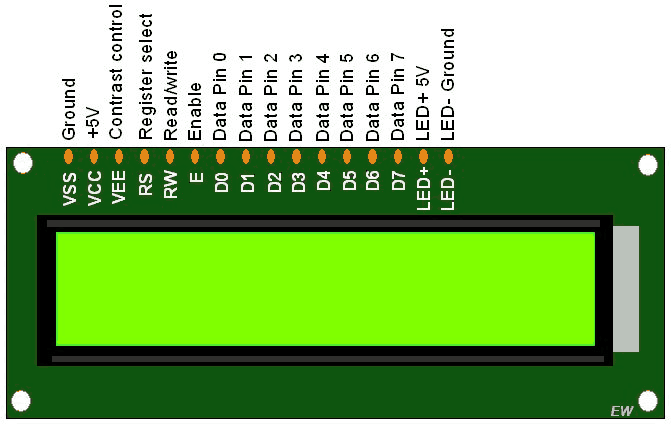
\includegraphics[width=0.7\linewidth]{figs/1.png}
\caption{LCD Display}
\label{fig:circuit}
\end{figure}

\subsection{LCD Connections}
\begin{center}
\begin{tabular}{|c|c|c|c|}
    \hline
    \textbf{LCD Pin} & \textbf{Function} & \textbf{Arduino Pin} & \textbf{Additional Components} \\
    \hline
    1 (VSS)  & Ground          & GND     & --- \\
    2 (VDD)  & Power Supply    & 5V      & --- \\
    3 (V0)   & Contrast Control &  180 $\Omega$ Resistor & Potentiometer (5k$\Omega$) \\
    4 (RS)   & Register Select  & D2      & --- \\
    5 (RW)   & Read/Write       & GND     & --- \\
    6 (E)    & Enable Signal    & D3      & --- \\
    7 (D0)   & Data Bit 0       & ---     & Not used \\
    8 (D1)   & Data Bit 1       & ---     & Not used \\
    9 (D2)   & Data Bit 2       & ---     & Not used \\
    10 (D3)  & Data Bit 3       & ---     & Not used \\
    11 (D4)  & Data Bit 4       & D4      & --- \\
    12 (D5)  & Data Bit 5       & D5      & --- \\
    13 (D6)  & Data Bit 6       & D6      & --- \\
    14 (D7)  & Data Bit 7       & D7      & --- \\
    15 (LED+) & Backlight Power  & 5V      & ---\\
    16 (LED-) & Backlight Ground & GND     & --- \\
    \hline
\end{tabular}
\end{center}

\subsection{Button Connections}

\begin{center}
\begin{tabular}{|c|c|c|}
    \hline
    \textbf{Button Index} & \textbf{Function} & \textbf{Arduino Pin} \\
    \hline
    0  & Button 0         & D8  \\
    1  & Button 1         & D9  \\
    2  & Button 2         & D10  \\
    3  & Button 3         & D11  \\
    4  & Button 4         & D12  \\
    5  & Button 5         & A0  \\
    6  & Button 6         & A1  \\
    7  & Button 7         & A2   \\
    8  & Button 8         & A3   \\
    9  & Button 9         & A4  \\
    Shift Button & Shift Mode       & A5    \\
    Extra Button & Extra Function   & D13   \\
    \hline
\end{tabular}
\end{center}


\section{Working Principle}
The Arduino processes inputs from the push buttons, performs arithmetic calculations, and displays the results on the LCD. It continuously monitors button presses to capture user input for numbers and operations. The software logic ensures correct mathematical operations and updates the display accordingly. Error handling mechanisms are also incorporated to manage invalid operations like division by zero.

\section*{Code Snippets}

\subsection*{Initialization and Setup}
\begin{lstlisting}[language=C, frame=single, basicstyle=\ttfamily\small, keywordstyle=\color{blue}]
#include <LiquidCrystal.h>
#include <Arduino.h>
#include <math.h>

#define PI 3.14159265358979323846

// LCD pins: RS, E, D4, D5, D6, D7
LiquidCrystal lcd(12, 11, 5, 4, 3, 2);

// Button configuration
const int buttons[] = {6, 7, 8, 9, 10, A0, A1, A2, A3, A4};
const int shiftButton = A5;
const int extraModeButton = 13;

void setup(){
  lcd.begin(16,2);
  Serial.begin(9600);
  
  // Setup buttons with internal pull-ups
  for(int i=0; i<10; i++){
    pinMode(buttons[i], INPUT_PULLUP);
  }
  pinMode(shiftButton, INPUT_PULLUP);
  pinMode(extraModeButton, INPUT_PULLUP);
  
  lcd.print("Calculator Ready");
  delay(1000);
  lcd.clear();
}
\end{lstlisting}

\subsection*{Main Loop and Button Handling}
\begin{lstlisting}[language=C, frame=single, basicstyle=\ttfamily\small, keywordstyle=\color{blue}]
void loop(){
  // Check mode buttons
  int currentShiftState = digitalRead(shiftButton);
  if(lastShiftState == HIGH && currentShiftState == LOW){
    shiftActive = true;
  }
  lastShiftState = currentShiftState;
  
  int currentExtraState = digitalRead(extraModeButton);
  if(lastExtraState == HIGH && currentExtraState == LOW){
    extraActive = true;
  }
  lastExtraState = currentExtraState;
  
  // Process number buttons
  for(int i=0; i<10; i++){
    if(digitalRead(buttons[i]) == LOW){
      delay(50); // debounce
      if(digitalRead(buttons[i]) == LOW){
        while(digitalRead(buttons[i]) == LOW);
        
        if(extraActive){
          if(i < 5) input += extraFuncs[i] + "(";
          else input += normalMode[i];
          extraActive = false;
        }
        else if(shiftActive){
          if(i < 6) handleSpecial(shiftOps[i]);
          else input += shiftFuncs[i - 6] + "(";
          shiftActive = false;
        }
        else{
          input += normalMode[i];
        }
        updateLCD();
      }
    }
  }
}
\end{lstlisting}

\subsection*{Display and Evaluation Functions}
\begin{lstlisting}[language=C, frame=single, basicstyle=\ttfamily\small, keywordstyle=\color{blue}]
void updateLCD(){
  lcd.clear();
  if(input.length() <= 16){
    lcd.print(input);
  }
  else{
    lcd.print(input.substring(0,16));
    lcd.setCursor(0,1);
    lcd.print(input.substring(16));
  }
}

float evaluateFullExpression(String expr){
  expr.trim();
  expr = processFunctions(expr);
  return evaluateExpression(expr);
}

float evaluateExpression(String expr){
  float result = 0.0;
  char lastOp = '+';
  String number = "";
  for(int i=0; i<expr.length(); i++){
    char c = expr.charAt(i);
    if(isDigit(c) || c == '.'){
      number += c;
    }
    else{
      float num = number.toFloat();
      number = "";
      switch(lastOp){
        case '+': result += num; break;
        case '-': result -= num; break;
        case '*': result *= num; break;
        case '/': result = (num!=0.0)? result/num:0.0; break;
      }
      lastOp = c;
    }
  }
  if(number.length() > 0){
    float num = number.toFloat();
    switch(lastOp){
      case '+': result += num; break;
      case '-': result -= num; break;
      case '*': result *= num; break;
      case '/': result = (num!=0.0)? result/num:0.0; break;
    }
  }
  return result;
}
\end{lstlisting}

\subsection*{Mathematical Function Approximations}
\begin{lstlisting}[language=C, frame=single, basicstyle=\ttfamily\small, keywordstyle=\color{blue}]
float mySin(float x){
  float rad = x * PI/180.0;
  while(rad > PI) rad -= 2*PI;
  while(rad < -PI) rad += 2*PI;
  float term = rad, sum = rad;
  for(int n=1; n<10; n++){
    term = -term * rad * rad/((2*n)*(2*n+1));
    sum += term;
  }
  return sum;
}

float myCos(float x){
  float rad = x * PI/180.0;
  while(rad > PI) rad -= 2*PI;
  while(rad < -PI) rad += 2*PI;
  float term = 1, sum = 1;
  for(int n=1; n<10; n++){
    term = -term * rad * rad/((2*n-1)*(2*n));
    sum += term;
  }
  return sum;
}

float mySqrt(float x){
  if(x < 0) return -1;
  float guess = x/2.0;
  for(int i=0; i<10; i++){
    guess = (guess + x/guess)/2.0;
  }
  return guess;
}

float myLn(float x){
  if(x<=0) return -1000000;
  float y = (x-1)/(x+1), sum = 0;
  for(int n=0; n<10; n++){
    sum += pow(y, 2*n+1)/(2*n+1);
  }
  return 2*sum;
}
\end{lstlisting}

\section{Results}
The implemented circuit successfully performed arithmetic operations using the scientific calculator. Inputs from the push buttons were accurately processed, and results were displayed on the LCD. Figure shows the actual implementation on a breadboard, demonstrating the calculator's ability to handle various operations, including addition, subtraction, multiplication, division, and advanced functions like trignometric inverse exponential and so on.

\section{Conclusion}
The experiment demonstrated the practical application of Arduino in designing a scientific calculator. The use of push buttons for input and an LCD display for output made the system user-friendly. Future improvements could include adding advanced mathematical functions, improving error handling, and optimizing the code for better performance.


\section{References}
\begin{enumerate}
\item Arduino Documentation: \texttt{https://www.arduino.cc/}
\item YouTube source
\end{enumerate}

\end{document}


